% Created 2017-01-08 Sun 16:28
% Intended LaTeX compiler: pdflatex
\documentclass[presentation,smaller]{beamer}
\RequirePackage{etex}
\RequirePackage[l2tabu,orthodox]{nag}            %% Warn about obsolete commands and packages
\RequirePackage{amsmath,amsfonts,amssymb,amsthm} %% Math
\RequirePackage{ifxetex,ifluatex}                %% Detect XeTeX and LuaTeX
\RequirePackage{fixltx2e}                        %% provides \textsubscript
\RequirePackage{xspace}
\RequirePackage{graphicx}
\RequirePackage{comment}
\RequirePackage{url}
\RequirePackage{relsize}
\RequirePackage{booktabs}
\RequirePackage{tabularx}
\RequirePackage[normalem]{ulem}
\RequirePackage[all]{xy}

%%%
%%% Code Listings
%%%

\RequirePackage{listings}
\lstdefinelanguage{Sage}[]{Python}{morekeywords={True,False,sage,cdef,cpdef,ctypedef,self},sensitive=true}

\lstset{frame=none,
  showtabs=False,
  showspaces=False,
  showstringspaces=False,
  commentstyle={\color{gray}},
  keywordstyle={\color{mLightBrown}\textbf},
  stringstyle ={\color{mDarkBrown}},
  frame=single,
  basicstyle=\tt\scriptsize\relax,
  backgroundcolor=\color{gray!190!black},
  inputencoding=utf8,
  literate={…}{{\ldots}}1,
  belowskip=0.0em,
}

%%%
%%% Tikz
%%%

\RequirePackage{tikz,pgfplots}

\usetikzlibrary{calc}
\usetikzlibrary{arrows}
\usetikzlibrary{automata}
\usetikzlibrary{positioning}
\usetikzlibrary{decorations.pathmorphing}
\usetikzlibrary{backgrounds}
\usetikzlibrary{fit,}
\usetikzlibrary{shapes.symbols}
\usetikzlibrary{chains}
\usetikzlibrary{shapes.geometric}
\usetikzlibrary{shapes.arrows}
\usetikzlibrary{graphs}

%% Cache

\ifdefined\tikzcaching  % chktex 1
  \usetikzlibrary{external}
  \tikzexternalize[prefix=build/]
  \tikzset{external/up to date check=diff}  %% MD5 fails from within emacs
\fi

%%%
%%% SVG (Inkscape)
%%%

\ifxetex % chktex 1
\newcommand{\executeiffilenewer}[3]{%
  {\immediate\write18{#3}} % hack
}
\else
\newcommand{\executeiffilenewer}[3]{%
  \ifnum\pdfstrcmp{\pdffilemoddate{#1}}%
    {\pdffilemoddate{#2}}>0%
    {\immediate\write18{#3}}
  \fi%
}
\fi

\newcommand{\includesvg}[2][1.0\textwidth]{%
 \executeiffilenewer{#1.svg}{#1.pdf}%
 {inkscape -z -D --file=#2.svg --export-pdf=#2.pdf --export-latex --export-area-page}%
 \def\svgwidth{#1} 
 \input{#2.pdf_tex}%
} 

%%%
%%% Metropolis Theme
%%%

\usetheme{metropolis}
\metroset{color/block=fill}
\metroset{numbering=none}
\metroset{outer/progressbar=foot}
\metroset{titleformat=smallcaps}

\setbeamercolor{description item}{fg=mLightBrown}
% \setbeamerfont{alerted text}{series=\bfseries}
\setbeamerfont{footnote}{size=\scriptsize}
\setbeamercolor{example text}{fg=mDarkBrown}

\renewcommand*{\UrlFont}{\ttfamily\smaller\relax}

%%%
%%% UTF-8
%%% 

\RequirePackage{unicodesymbols} % after metropolis which loads fontspec

%%%
%%% BibLaTeX
%%%

\RequirePackage[backend=bibtex,
            style=alphabetic,
            maxnames=4,
            citestyle=alphabetic]{biblatex}

\bibliography{local.bib,abbrev3.bib,crypto_crossref.bib,rfc.bib,jacm.bib}

\DeclareFieldFormat{title}{\alert{#1}}
\DeclareFieldFormat[book]{title}{\alert{#1}}
\DeclareFieldFormat[thesis]{title}{\alert{#1}}
\DeclareFieldFormat[inproceedings]{title}{\alert{#1}}
\DeclareFieldFormat[incollection]{title}{\alert{#1}}
\DeclareFieldFormat[article]{title}{\alert{#1}}
\DeclareFieldFormat[misc]{title}{\alert{#1}}

%%% 
%%% Microtype
%%%

\IfFileExists{upquote.sty}{\RequirePackage{upquote}}{}
\IfFileExists{microtype.sty}{\RequirePackage{microtype}}{}

\setlength{\parindent}{0pt}                   %%
\setlength{\parskip}{6pt plus 2pt minus 1pt}  %%
\setlength{\emergencystretch}{3em}            %% prevent overfull lines
\setcounter{secnumdepth}{0}                   %%

%%% Local Variables:
%%% mode: latex
%%% End:
\usepackage{graphicx}
\usepackage{grffile}
\usepackage{longtable}
\usepackage{wrapfig}
\usepackage{rotating}
\usepackage[normalem]{ulem}
\usepackage{amsmath}
\usepackage{textcomp}
\usepackage{amssymb}
\usepackage{capt-of}
\usepackage{hyperref}
\usepackage{microtype}
\usepackage{newunicodechar}
\usepackage{unicodesymbols}
\usepackage[notions,operators,sets,keys,ff,adversary,primitives,complexity,asymptotics,lambda,landau]{cryptocode}
\usepackage{xspace}
\usepackage{units}
\usepackage{nicefrac}
\usepackage{gensymb}
\usepackage{amsthm}
\usepackage{amsmath}
\usepackage{amssymb}
\usepackage{xcolor}
\usepackage{listings}
\usepackage[color=yellow!40]{todonotes}
\newcommand{\ZZ}[1][blank]{\ensuremath{\ifthenelse{\equal{#1}{blank}}{\mathbb{Z}}{\mathbb{Z}\left[#1\right]}\xspace}}
\newcommand{\QQ}[1][blank]{\ensuremath{\ifthenelse{\equal{#1}{blank}}{\mathbb{Q}}{\mathbb{Q}\left[#1\right]}\xspace}}
\newcommand{\ZZq}[1][blank]{\ensuremath{\ifthenelse{\equal{#1}{blank}}{\mathbb{Z}_q}{\mathbb{Z}_q\left[#1\right]}\xspace}}
\renewcommand{\U}[1]{\ensuremath{\mathcal{U}\left( {#1} \right)}\xspace}
\newcommand{\mat}[1]{\ensuremath{\mathbf{#1}}\xspace}
\renewcommand{\vec}[1]{\ensuremath{\mathbf{#1}}\xspace}
\newcommand{\sample}{\ensuremath{\leftarrow_{\$}}}
\definecolor{lightblue}{HTML}{4B8EC8}
\usetheme{default}
\author{Martin R. Albrecht \texttt{@martinralbrecht}}
\date{15 June 2016 — Bletchley Park}
\title{Learning with Errors}
\subtitle{Post-Quantum Candidates from Noisy Linear Systems}
\hypersetup{
pdfauthor={Martin R. Albrecht \texttt{@martinralbrecht}},
pdftitle={Learning with Errors},
pdfkeywords={},
pdfsubject={},
pdfcreator={Emacs 25.1.1 (Org mode 9.0.3)},
pdflang={English},
colorlinks,
citecolor=gray,
filecolor=gray,
linkcolor=gray,
urlcolor=gray
}
\begin{document}

\maketitle
\begin{frame}{Outline}
\tableofcontents
\end{frame}


\section{Motivation}
\label{sec:org9621948}

\begin{frame}[fragile,label={sec:orgdb9f820}]{A Typical Scenario}
 \lstset{language=plantuml,label= ,caption= ,captionpos=b,numbers=none}
\begin{lstlisting}
skinparam monochrome true
skinparam dpi 600
skinparam backgroundColor transparent
skinparam classBackgroundColor transparent
skinparam style strictuml
skinparam handwritten true
skinparam packageStyle rect
skinparam defaultFontName FG Virgil

activate Client
Client -> Server: g<sup>a</sup>
activate Server
Client <- Server: g<sup>b</sup>, sign<sub>sk</sub>(g<sup>b</sup>)
note left: K= g<sup>ab</sup>
Client -> Server: E<sub>K</sub>(data)
note right: K= g<sup>ab</sup>
Server --> Client: E<sub>K</sub>(more data)
deactivate Server
deactivate Client
\end{lstlisting}

\begin{center}
\begin{center}
\includegraphics[width=0.5\textwidth]{key exchange.png}
\end{center}
\end{center}

\begin{itemize}
\item \(g^a\), \(g^b\), \(g^{ab}\) is a \alert{Diffie-Hellman} triple
\item sign\(_{sk}(⋅)\) typically realised using \alert{RSA} signatures
\end{itemize}
\end{frame}

\begin{frame}[label={sec:org1437367}]{Bye, bye DDH and RSA (?)}
\begin{center}
Both problems are easy on quantum computers
\end{center}

\pause

\begin{itemize}[<+->]
\item \fullcite{ETSI:PQ15}
\item \fullcite{NSA:PQ15}
\item \fullcite{CESG:PQ16}
\end{itemize}
\end{frame}


\begin{frame}[label={sec:orgf7b0cfd}]{Hello Post-Quantum}
\begin{center}
\begin{center}
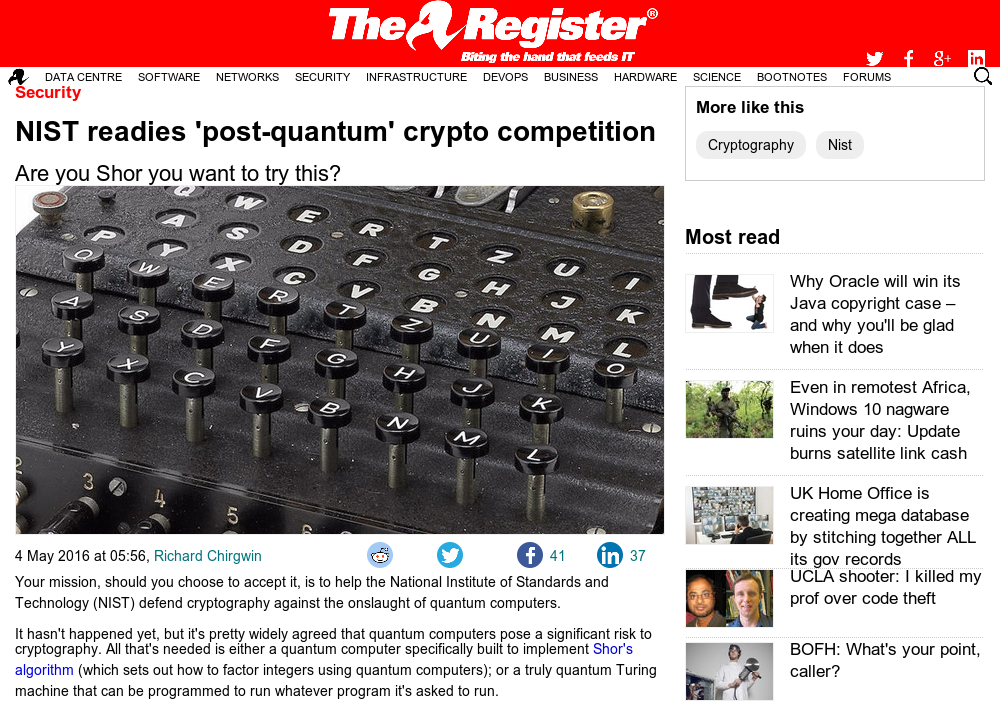
\includegraphics[width=.9\linewidth]{./competition.png}
\end{center}
\end{center}
\end{frame}


\begin{frame}[label={sec:orgf00203b}]{Post-Quantum Families}
\begin{itemize}
\item Multivariate Quadratic Cryptography
\item Code-based Cryptography
\item Hash-based Signatures
\item \alert<2->{Lattice-based Cryptography}
\end{itemize}
\end{frame}

\section{Learning with Errors}
\label{sec:org4bac775}

\begin{frame}[label={sec:org8b2c2ec}]{Linear System Solving}
Given \((\vec{A},\vec{c})\) with \(\vec{c} \in \ZZq^{m}\), \(\vec{A} \in \ZZq^{m × n}\) and \(\vec{s} \in \ZZq^{n}\) is

\[
\left(\begin{array}{c}
\\
\\
\\ 
\vec{c} \\
\\
\\
\\
\end{array} \right) = \left(
\begin{array}{ccc}
\leftarrow & n & \rightarrow \\
\\
\\ 
& \vec{A} & \\
\\
\\
\\
\end{array} \right) \times \left( \begin{array}{c}
\\
\vec{s} \\
\\
\end{array} \right)
\]

or \(\vec{c} \sample \U{\ZZq^{m}}\).
\end{frame}


\begin{frame}[label={sec:org072e156}]{Learning with Errors}
Given \((\vec{A},\vec{c})\) with \(\vec{c} \in \ZZq^{m}\), \(\vec{A} \in \ZZq^{m × n}\), \(\vec{s} \in \ZZq^{n}\) and \alert{small \(\vec{e} \in \ZZ^{m}\)} is

\[
\left(\begin{array}{c}
\\
\\
\\ 
\vec{c} \\
\\
\\
\\
\end{array} \right) = \left(
\begin{array}{ccc}
\leftarrow & n & \rightarrow \\
\\
\\ 
& \vec{A} & \\
\\
\\
\\
\end{array} \right) \times \left( \begin{array}{c}
\\
\vec{s} \\
\\
\end{array} \right) \alert{+ \left(
\begin{array}{c}
\\
\\
\\ 
\vec{e} \\
\\
\\
\\
\end{array} 
\right)}
\]

or \(\vec{c} \sample \U{\ZZq^{m}}\).
\end{frame}


\begin{frame}[label={sec:org3159ad1}]{Parameters}
\begin{columns}
\begin{column}{0.5\columnwidth}
\begin{tikzpicture}[scale=0.7]
  \begin{axis}[
    domain=-10:10,
    grid=major,smooth,
    xlabel=$x$,
    ylabel=$\approx \textnormal{Pr}(x)$,
    ]
    \addplot[color=mLightBrown,very thick,samples=50,smooth]{exp(-(x^2)/18)};
    \addplot[only marks,color=lightblue] coordinates {
      (-9, 0.011)
      (-8, 0.028)
      (-7, 0.065)
      (-6, 0.135)
      (-5, 0.249)
      (-4, 0.411)
      (-3, 0.606)
      (-2, 0.800)
      (-1, 0.945)
      (0, 1.000)
      (1, 0.945)
      (2, 0.800)
      (3, 0.606)
      (4, 0.411)
      (5, 0.249)
      (6, 0.135)
      (7, 0.065)
      (8, 0.028)
      (9, 0.011)
    };
  \end{axis}
\end{tikzpicture}
\end{column}


\begin{column}{0.5\columnwidth}
\begin{itemize}
\item Parameters are: 
\begin{itemize}
\item dimension \(n\),
\item modulus \(q\) (e.g. \(q \approx n^2\)),
\item noise size \(\alpha\) (e.g. \(\alpha q \approx \sqrt{n}\)),
\item number of samples \(m\).
\end{itemize}

\item Elements of \(\vec{A}, \vec{s}, \vec{e}, \vec{c}\) are in \(\ZZ_q\).
\item \(\vec{e}\) is sampled from \(χ_{α}\), a discrete Gaussian with width \[\sigma=\frac{\alpha q}{\sqrt{2 \pi}}.\]
\end{itemize}
\end{column}
\end{columns}
\end{frame}


\begin{frame}[label={sec:orgd1aa6e2}]{Lattices}
\begin{itemize}
\item A lattice is a discrete additive subgroup of \(\mathbb{R}^n\).

\item Let \(\vec{B} = \{ \vec{b}_1, \ldots, \vec{b}_n \}\) be \(m\) linearly independent vectors in \(\mathbb{R}^n\). Then \(L(\vec{B})=\{ \sum_{i=1}^{n} x_i \vec{b}_i \,|\, x_i \in \ZZ\}\) is the lattice generated by \(\vec{B}\).
\end{itemize}

\begin{center}
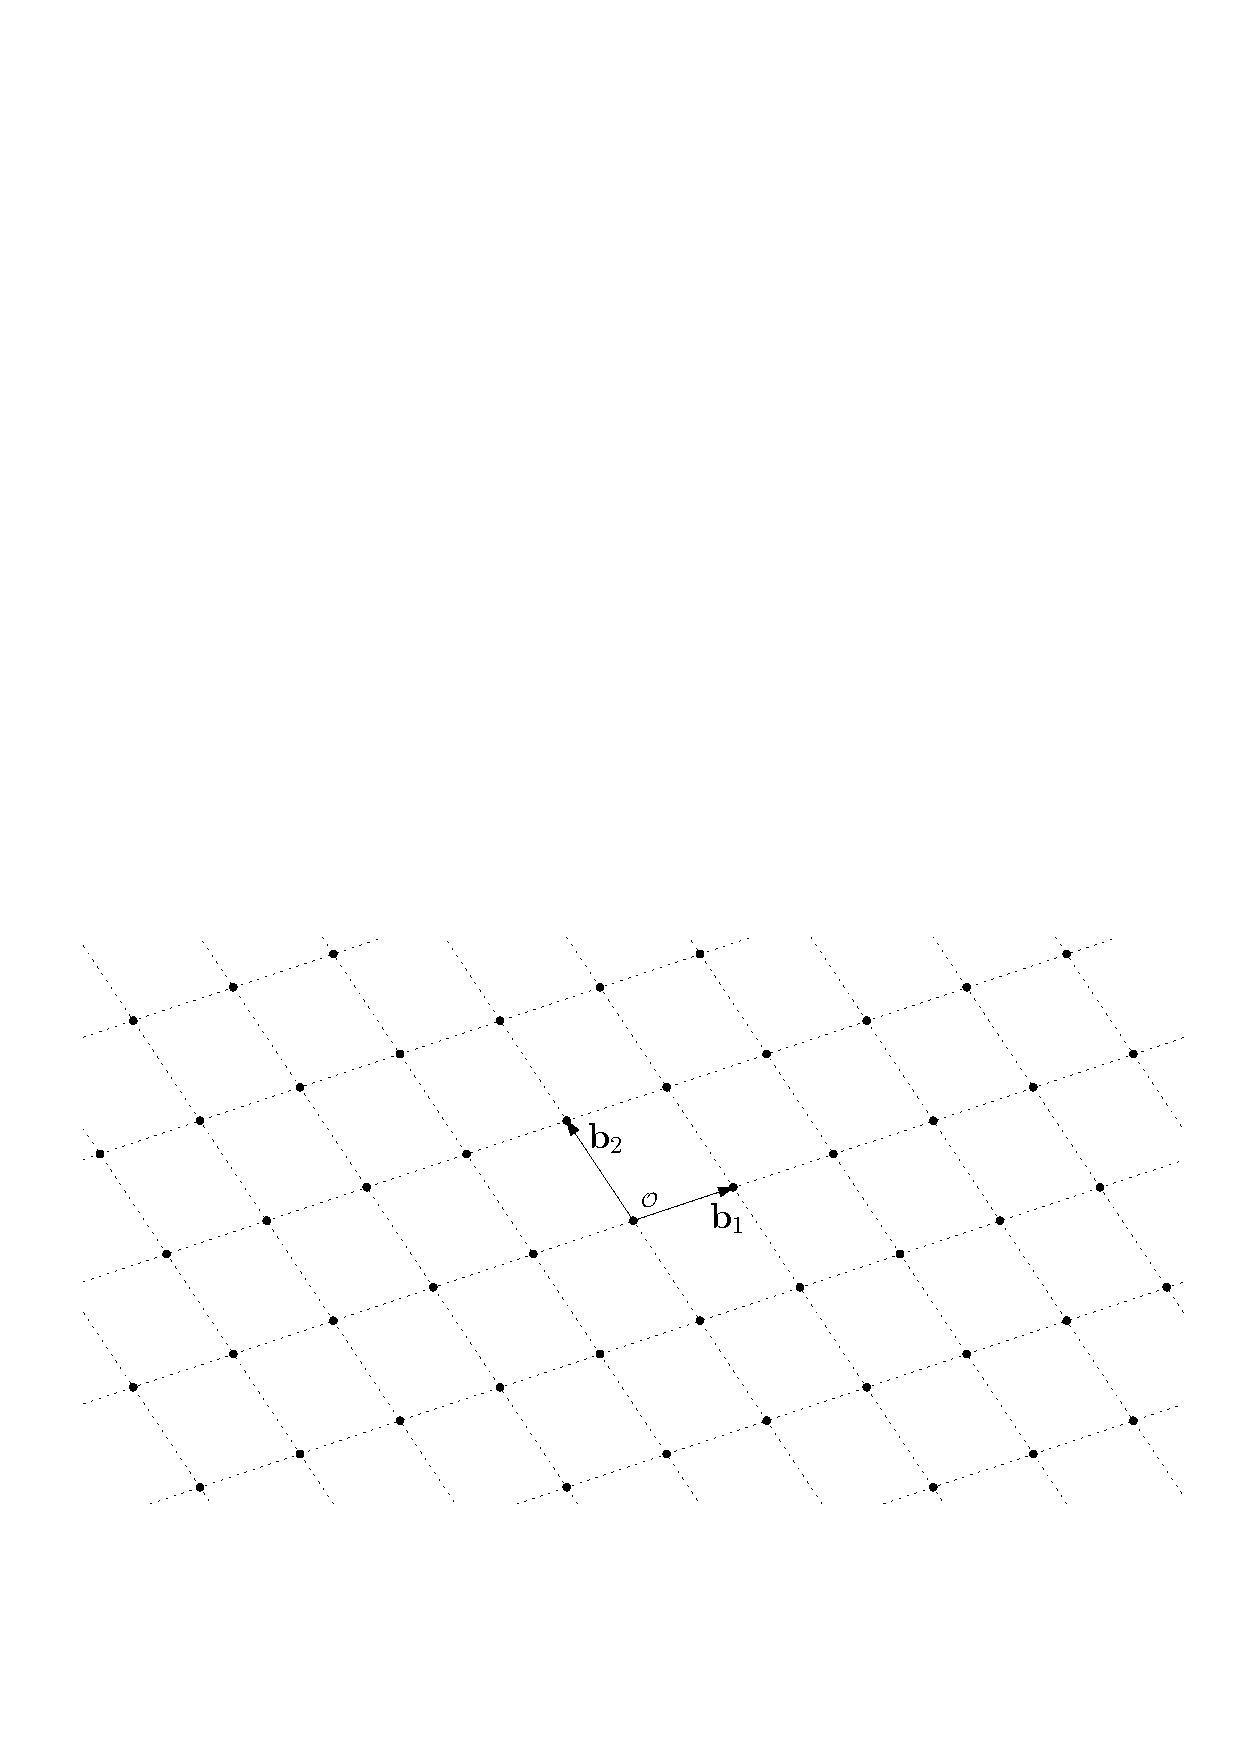
\includegraphics[width=.9\linewidth]{./joop-latt1.pdf}
\end{center}

\tiny Picture Credit: Joop van der Pol
\end{frame}


\begin{frame}[label={sec:org672584c}]{Bounded Distance Decoding}
Let \(\vec{B} = [\vec{A} | q\vec{I}]^T\). LWE = BDD for \(\vec{c}\) and \(L(\vec{B})\).

\begin{center}
\includegraphics[width=.9\linewidth]{./joop-cvp.pdf}
\end{center}

\tiny Picture Credit: Joop van der Pol
\end{frame}


\begin{frame}[label={sec:org00d448d}]{Shortest Vector Problem}
\begin{description}
\item[{SVP}] Find the shortest non-zero vector in \(L(\vec{B})\)
\item[{GapSVP\(_γ\)}] return YES if \(λ_1(L(\vec{B})) ≤ d\), and NO if \(λ_1(L(\vec{B})) > γ⋅d\).
\end{description}

\begin{center}
\begin{center}
\includegraphics[width=.9\linewidth]{./joop-l1.pdf}
\end{center}
\end{center}

\tiny Picture Credit: Joop van der Pol
\end{frame}

\begin{frame}[label={sec:org27e262e}]{Good and Bad Bases}
With a “good basis” many lattice problems are easy.

\begin{center}
\begin{center}
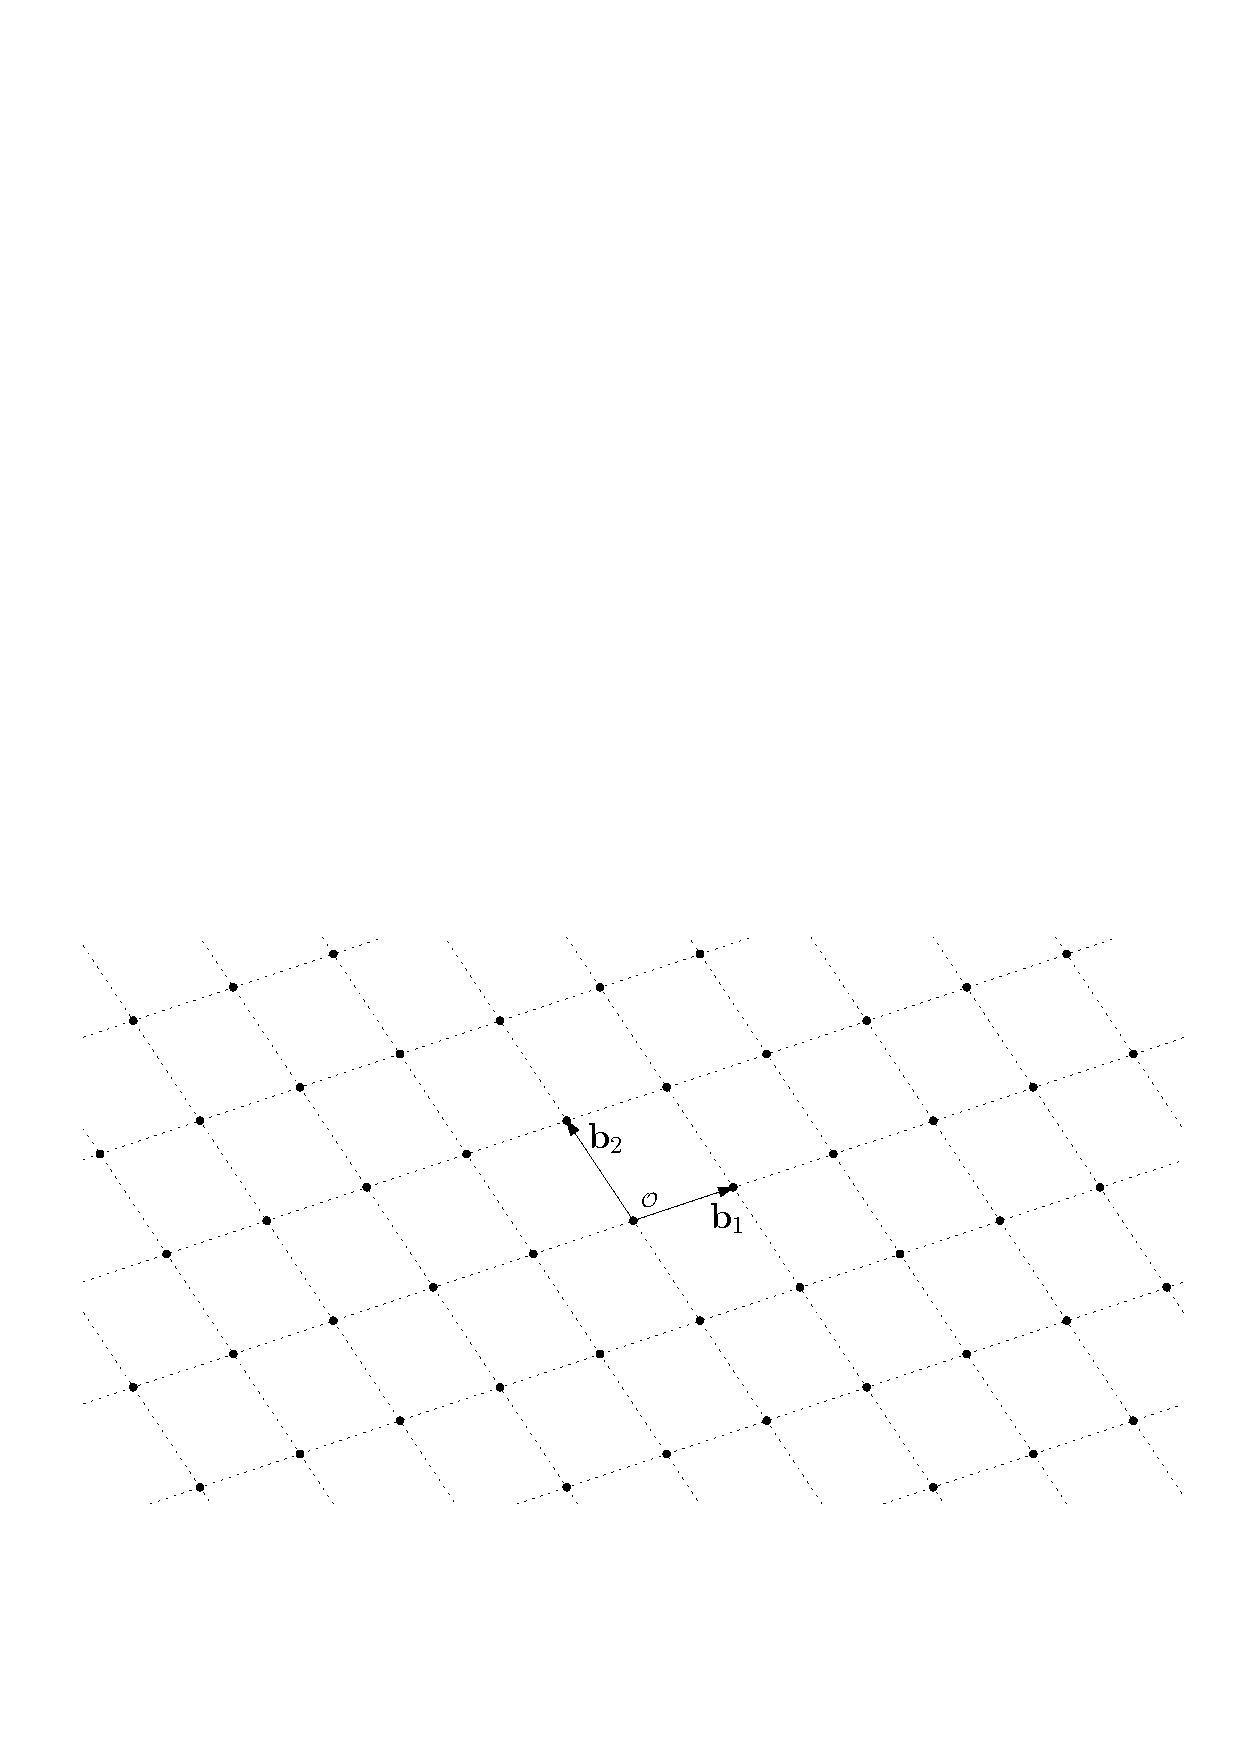
\includegraphics[width=.9\linewidth]{./joop-latt1.pdf}
\end{center}
\end{center}

\tiny Picture Credit: Joop van der Pol
\end{frame}


\begin{frame}[label={sec:org59a9dc6}]{Good and Bad Bases}
With “bad basis” GapSVP\(_γ\) for polynomial \(γ\) assumed exponential.

\begin{center}
\begin{center}
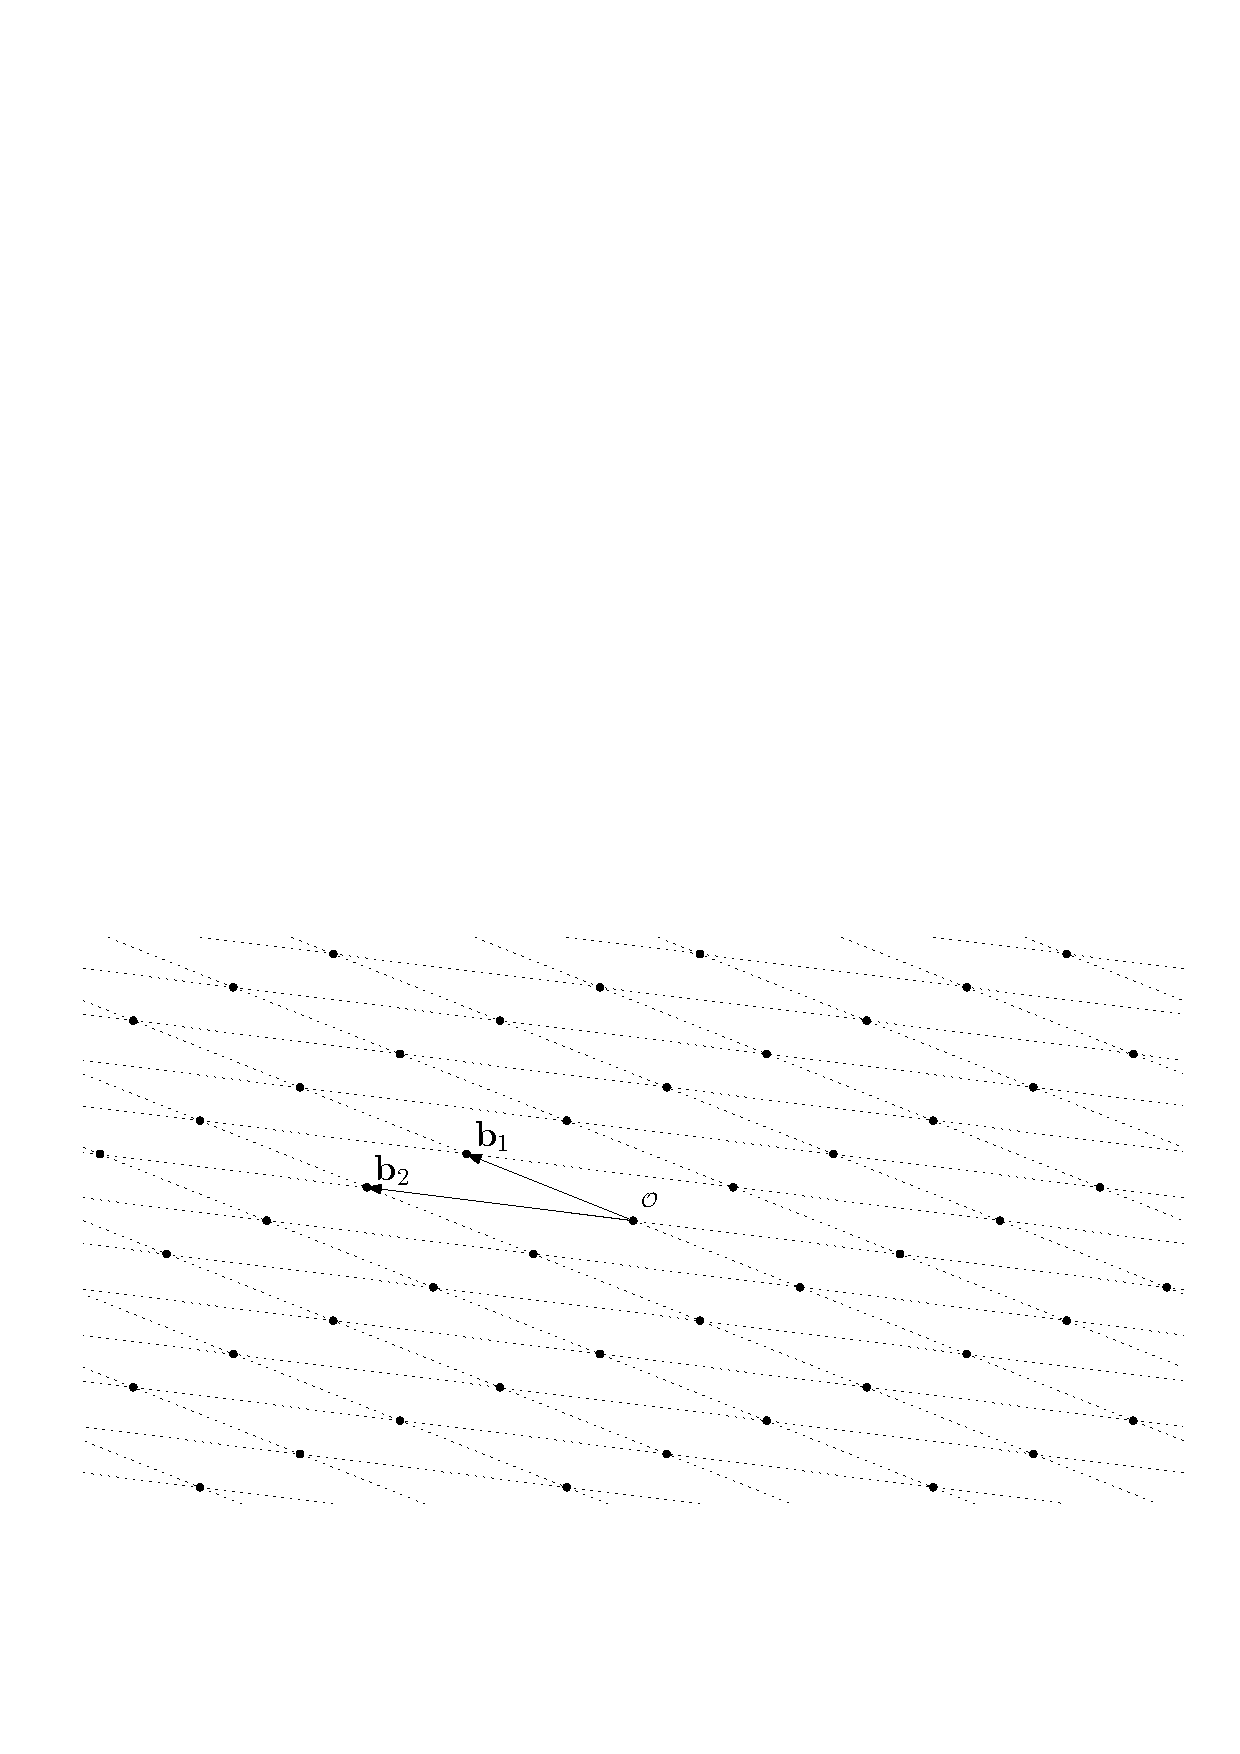
\includegraphics[width=.9\linewidth]{./joop-latt2a.pdf}
\end{center}
\end{center}

\tiny Picture Credit: Joop van der Pol
\end{frame}


\begin{frame}[label={sec:orgf6824dd}]{Regev’s Reduction}
\begin{theorem}
\begin{itemize}
\item Let \(e\) follow \(χ_α\), a (discrete) Gaussian distribution over \(\ZZ\) with standard deviation \(σ = \frac{α\, q}{\sqrt{2π}}\).
\item If \(σ >  \sqrt{n}\), worst-case GapSVP\(_{\tilde{\mathcal{O}}(n/α)}\) reduces to average-case LWE.
\end{itemize}
\end{theorem}

\fullcite{STOC:Regev05}
\end{frame}


\begin{frame}[label={sec:orgd4bfd18}]{Encryption}
\begin{description}
\item[{Public Key}] \(\vec{A},\vec{c}\) with \(\vec{c} = \vec{A}\cdot \vec{s} + \vec{e}\)
\item[{Secret Key}] \(\vec{s}\)
\item[{Encrypt}] \(\vec{b} \sample \{0,1\}^m\) and return \((\vec{a}',c')\) with \(\vec{a}' = \vec{b} \cdot \vec{A}\), \(c' = \langle \vec{b}, \vec{c} \rangle + m \cdot \lfloor q/2\rfloor + e'\) for \(m \in \{0,1\}\)

\item[{Decrypt}] \(c' - \langle \vec{a}', \vec{s} \rangle = \vec{b} \cdot \vec{A} \cdot \vec{s} + \langle \vec{b}, \vec{e} \rangle + \lfloor q/2 \rfloor \cdot m + e' -  \vec{b} \cdot \vec{A} \cdot \vec{s}\)
\end{description}
\end{frame}

\begin{frame}[label={sec:org71d7424}]{Key Exchange: LWE Normal Form}
Given an LWE instance with \(\vec{s} \sample \U{\ZZ_q^n}\), we can construct samples of the form \((\vec{a}, \langle \vec{a}, \vec{s}'\rangle+e)\) with \(s_i'\) sampled from the distribution of \(e\).

\begin{itemize}
\item Take \(n\) rows and write \((\vec{A}, \vec{c}) = (\vec{A}, \vec{A}⋅\vec{s} + \vec{e})\).

\item With good probability \(\vec{A}\) is invertible.

\item Get a row \((\vec{a}', c') = (\vec{a}', \langle \vec{a}', \vec{s}\rangle + e')\) and compute \footfullcite{C:ACPS09} \[\vec{a}'⋅ \vec{A}^{-1} ⋅ \vec{c}-c' = \vec{a}' ⋅ \vec{A}^{-1} (\vec{A}⋅ \vec{s}+\vec{e}_0)- \vec{a}'·\vec{s}-e_1 = \vec{a}' ⋅ \vec{A}^{-1} ⋅ \vec{e} - e'.\]

\item \((\vec{a}' ⋅ \vec{A}^{-1},\  \vec{a}'⋅ \vec{A}^{-1} ⋅ \vec{c}-c')\) is your new sample.
\end{itemize}
\end{frame}


\begin{frame}[label={sec:orge9efbdd}]{Key Exchange \footfullcite{SP:BCNS15,EPRINT:ADPS15}}
\begin{description}
\item[{Alice}] samples \(\vec{A},\vec{c}_a=\vec{A}\cdot \vec{s}_a + \vec{e}_a\) with \(\vec{s}_a \sample χ_α^n\)  \\
sends \((\vec{A},\vec{c})\)
\item[{Bob}] samples \(\vec{c}_b=\vec{s}_b \cdot \vec{A} + \vec{e}_b\) with \(\vec{s}_b \sample χ_α^n\) \\
sends \(\vec{c}_b\)
\end{description}

\begin{block}{Shared Secret}
\[\vec{s}_b \cdot (\vec{A} \cdot \vec{s}_a + \vec{e}_a) \approx (\vec{s}_b \cdot \vec{A} + \vec{e}_a) \cdot \vec{s}_a \approx \vec{s}_b \cdot \vec{A} \cdot \vec{s}_a\]
\end{block}
\end{frame}

\begin{frame}[label={sec:orgada35b3}]{Signatures (from SIS)}
\begin{block}{SIS}
Given \(\vec{A} \in \mathbb{Z}_q^{m \times n}\) find \alert{small} \(\vec{s}\) such that \(\vec{s}⋅\vec{A} = 0\) 
\end{block}

\begin{itemize}
\item Hash-and-Sign signatures \footfullcite{STOC:GenPeiVai08}

\item Fiat-Shamir signatures \footfullcite{C:DDLL13}
\end{itemize}
\end{frame}



\section{Challenges}
\label{sec:org4ea51c0}

\begin{frame}[label={sec:orgf28b335}]{Regev’s Reduction}
\begin{itemize}
\item<1-> An algorithm solving LWE 
\begin{itemize}
\item for a fraction \(1/n^{d_1}\)
\item with advantage \(1/n^{d_2}\)
\item given \(m = n^c\) samples
\end{itemize}
implies a polynomial-time algorithm solving GapSVP\(_γ\) calling LWE solving oracle \(\mathcal{O}(n^{11+c+d_1+2d_2})\) times.\footfullcite{EPRINT:CKMS16}

\item<2-> “Solving LWE \(n^{11+}\) times is hard”

\item<3-> Best Known Attacks on LWE: \(2^{\mathcal{O}(n)}\) time \textbf{and} \(2^{\mathcal{O}(n)}\) memory
\end{itemize}
\end{frame}

\begin{frame}[label={sec:org8c1f772}]{How Hard is \(2^{\mathcal{O}(n)}\) Time and \(2^{\mathcal{O}(n)}\) Memory?}
\begin{itemize}
\item How big should we choose \(n\), \(q\) and the noise?
\item Many problem formulations: SIS, BDD, uSVP, …
\item Many algorithms: combinatorial, algebraic, geometric
\item Quantum attacks
\end{itemize}

\fullcite{JMC:AlbPlaSco15}
\end{frame}

\begin{frame}[label={sec:org4d28eb8}]{Lattice Reduction}
\begin{columns}
\begin{column}{0.4\columnwidth}
\begin{itemize}
\item Practically relevant algorithms rely on \alert{lattice reduction} as a subroutine.
\item Concrete performance of lattice reduction algorithms is not well understood.
\end{itemize}
\end{column}

\begin{column}{0.6\columnwidth}
\begin{tikzpicture}
\begin{axis}[domain=0:80,grid=major,smooth,xlabel=dimension,width=0.9\textwidth,height=0.5\textheight,
ylabel=SVP running time in $s$,]
\addplot[color=mLightBrown,very thick,smooth] coordinates {
( 3,  0.000910) ( 4,  0.000909) ( 5,  0.000936) ( 6,  0.000980) ( 7,  0.001024)
( 8,  0.001131) ( 9,  0.001141) (10,  0.001202) (11,  0.001270) (12,  0.001350)
(13,  0.001437) (14,  0.001540) (15,  0.001715) (16,  0.001806) (17,  0.001963)
(18,  0.002104) (19,  0.002211) (20,  0.002387) (21,  0.002614) (22,  0.002912)
(23,  0.003123) (24,  0.003419) (25,  0.003757) (26,  0.004183) (27,  0.004732)
(28,  0.005179) (29,  0.005966) (30,  0.006723) (31,  0.007673) (32,  0.008967)
(33,  0.011072) (34,  0.015257) (35,  0.013562) (36,  0.014296) (37,  0.017413)
(38,  0.021087) (39,  0.023248) (40,  0.021857) (41,  0.042012) (42,  0.032311)
(43,  0.036711) (44,  0.037855) (45,  0.054784) (46,  0.065419) (47,  0.083879)
(48,  0.082325) (49,  0.110854) (50,  0.120147) (51,  0.220014) (52,  0.143344)
(53,  0.191638) (54,  0.331177) (55,  0.236328) (56,  0.268762) (57,  0.506213)
(58,  0.534709) (59,  0.697577) (60,  0.748292) (61,  0.868768) (62,  1.125313)
(63,  1.744673) (64,  1.846011) (65,  2.368306) (66,  2.433754) (67,  3.704405)
(68,  4.205946) (69,  5.492047) (70,  5.995138) (71,  8.296805) (72,  9.878952)
(73, 13.587996) (74, 15.478631) (75, 23.804719) (76, 25.346042) (77, 41.266405)
(78, 46.407407) (79, 73.522041) (80, 86.350488)
};   
\end{axis}
\end{tikzpicture}
\end{column}
\end{columns}

\begin{block}{Software}
\begin{itemize}
\item \url{https://github.com/dstehle/fplll}
\item \url{https://github.com/malb/fpylll}
\item \url{http://perso.ens-lyon.fr/gilles.villard/hplll/}
\end{itemize}
\end{block}
\end{frame}


\begin{frame}[label={sec:org0a34fc6}]{Performance}
\begin{itemize}
\item \alert{Computational} cost for LWE is quite manageable because it only involves simple linear operations over \(\mathbb{Z}_q\) where \(q\) can be word-sized.
\item Public-key and ciphertext \alert{sizes} can be prohibitively expensive: \(\mathcal{O}(n^2 \log_2 q)\) and \(\mathcal{O}(n \log_2 q)\)
\end{itemize}

\begin{block}<2->{Rule of Thumb}
Post-quantum schemes are not slow, but they are big.
\end{block}
\end{frame}

\begin{frame}[label={sec:orgf16b4b0}]{Better Performance: Ring-LWE}
\begin{itemize}
\item Replace random \(\vec{A}\) by structured matrices, e.g. cyclic or nega-cyclic matrices.
\item This is equivalent to computing in \(\ZZ_q[x]/P(x)\).
\item The problem is then called \alert{Ring-LWE}.
\end{itemize}

\pause

\begin{block}{No Silver Bullet}
\(n=1024, q≈ 2^{14} →\) 1792 bytes vs. MTU of 1500 bytes in Ethernet.
\end{block}
\end{frame}

\begin{frame}[label={sec:orgd9f7dd2}]{Rings: Not all Problems are Hard}
\begin{itemize}
\item Let \(n=2^k\), sample some small \(g ∈ \ZZ[x]/(x^n+1)\).
\item Consider the matrix \(\vec{G}\) spanned by the coefficient vectors of \(\{x^i \cdot g \bmod x^n+1\}\).
\item Compute the Hermite normal form  \(\vec{H} = \textnormal{HNF}(\vec{G})\).
\item With good probability \(g\) is a shortest vector of the lattice \(L(\vec{H})\).
\end{itemize}

Finding \(g\) takes polynomial time on a quantum computer.\footfullcite{CamGroShe14,EC:CDPR15}
\end{frame}

\begin{frame}[label={sec:org2302be4}]{Rings: Not all Problems are as Hard}
\begin{itemize}
\item What if \(\ZZq[x]/P(x)\) has subfields?
\item Distinguishing \(h = f/g \in \ZZ_q[x]/P(x)\) from random for small \(f\) and \(g\) and big \(q\) is easier than expected.\footfullcite{EC:GenSzy02,EPRINT:AlbBaiDuc16}
\end{itemize}
\end{frame}

\begin{frame}[label={sec:org82d6268}]{Rings: No Known Attacks}
There is \alert{no known attack} which successfully exploits ring structure for properly chosen Ring-LWE parameters.
\end{frame}

\begin{frame}[label={sec:org739fcf5}]{CCA Security}
\begin{itemize}
\item The schemes described here (and in the literature) promise IND-CPA security, i.e. security against chosen-plaintext attacks.
\item They do not promise IND-CCA security, i.e. security against chosen-ciphertext attacks.
\item Building efficient CCA secure schemes from LWE is still open.\footfullcite{STOC:Peikert09}
\end{itemize}
\end{frame}

\begin{frame}[label={sec:org719d981}]{Fin}
\begin{center}
\begin{Large}
\alert{Thank You}
\end{Large}
\end{center}
\end{frame}
\end{document}